\section{Closed-loop Model Checking Using the Abstraction Tree}
After the abstraction tree is built, it can be used for closed-loop model checking by non-domain experts. 
The question is which models to select from the abstraction tree to perform model checking, and provide the most concrete counter-examples, possibly under multiple physiological conditions, for the physicians to determine the validity of the counter-examples. %\cite{uppaal}

Recall the definition of appropriateness from Section \ref{preliminaries}.
In the technical report \cite{regar_tech}, we show that a sufficient condition for a model $M$ to be appropriate for a requirement $\varphi$ with monitor $Mon$ is
\[Var(\varphi) \subset Var(M) \cup Var(Mon)\].

Algorithm 1 (\figref{algorithm}) selects the most abstract models from the abstraction tree $HM\_tree$ that are appropriate for a requirement $Req$.
\begin{figure}[!t]
		\centering
		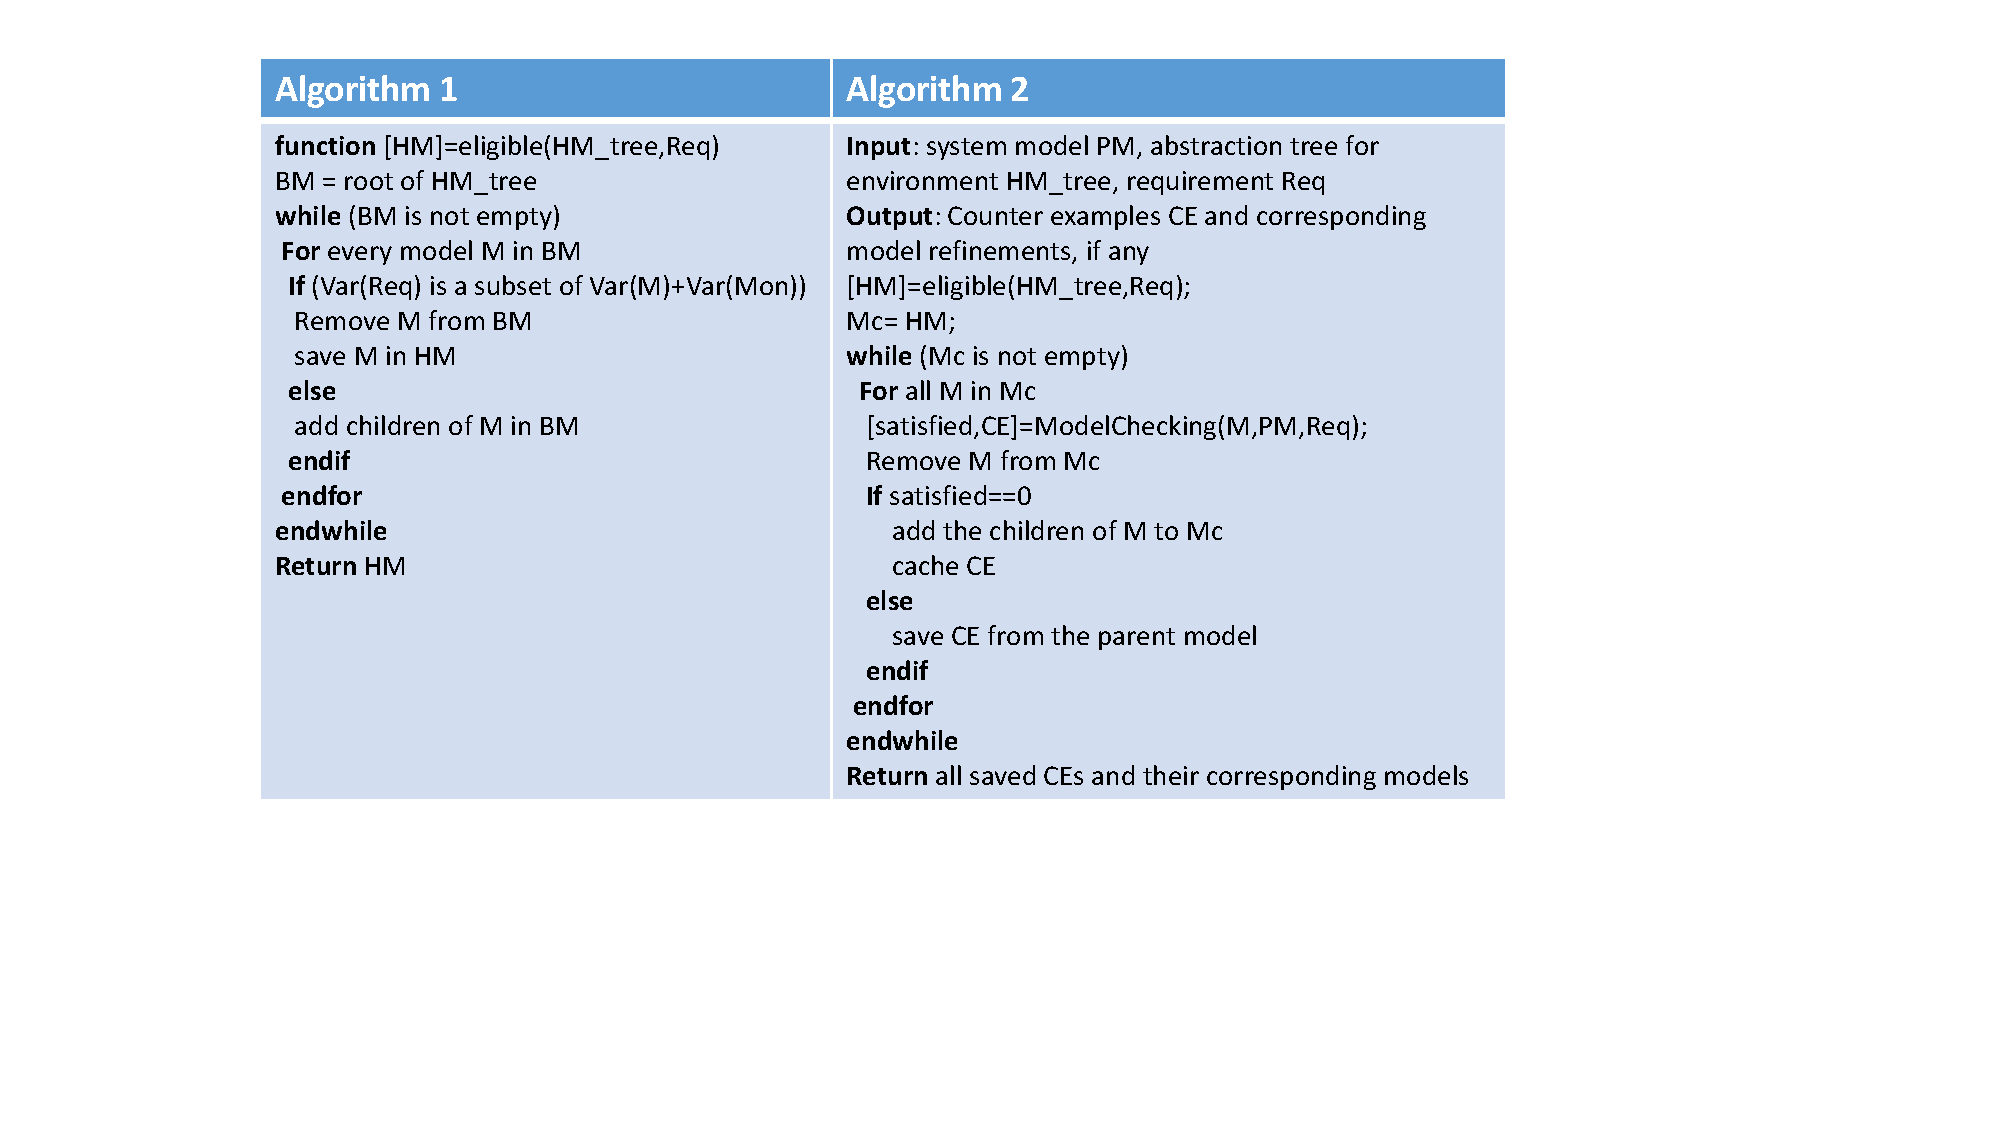
\includegraphics[width=0.9\textwidth]{figs/algorithm.pdf}
		%\vspace{-5pt}
		\caption{\small Algorithms for closed-loop model checking with abstraction tree}
		  \vspace{-10pt}
		\label{fig:algorithm}
\end{figure}

Upon requirement violation, an abstract counter-example is returned during closed-loop model checking. The counter-example may contain context ambiguities that should be resolved before sending to the physician. An abstraction tree contains the information of how different environment conditions are over-approximated by more abstract models. By exploring the abstraction tree, the most concrete yet unambiguous counter-examples can be sent to the physicians for analysis. Algorithm 2 (\figref{algorithm}) describes the process for closed-loop model checking with an abstraction tree.



%The most abstract model in the abstraction tree is built to cover the input space to the device as much as possible, thus it may not have enough details to constrain the behaviors of the model according to the constraints in the requirement. Thus the first step of closed-loop model checking is to select the most abstract models which are appropriate for the requirement. A model $M$ is appropriate for a requirement $Req$ if the environment transitions mentioned in the requirement, denoted as $EnvT(Req)$, is a subset of the environment transitions associated with the model $EnvT(M$). The following algorithm finds the most abstract heart models in the abstraction tree $HM\_tree$ that are appropriate for a requirement $Req$.
%\begin{Verbatim}
%Algorithm 1
%function [HM]=eligible(HM_tree,Req)
%BM = root of HM_tree
%while (BM is not empty)
 %For every model M in BM
  %If (Var(Req) is a subset of Var(M)+Var(Mon))
   %Remove M from BM
   %save M in HM
  %else
   %add children of M in BM
  %endif
 %endfor
%endwhile
%Return HM
%\end{Verbatim}
%BM = all models in HM_tree with all Prop(Req)
%For all M in BM
 %while (in the parent of M no behavior in Prop(Req) is abstracted with other behaviors)
	 %M = parent of M
 %endwhile
 %save M in HM
 %endfor

%\begin{Verbatim}
%Algorithm 2
%Input: system model PM, abstraction tree for environment HM_tree, requirement Req
%Output: Counter examples CE and corresponding model refinements, if any
%[HM]=eligible(HM_tree,Req);
%Mc= HM;
 %while (Mc is not empty)
  %For all M in Mc
   %[satisfied,CE]=ModelChecking(M,PM,Req);
	 %Remove M from Mc
	 %If satisfied==0
	  %add the children of M to Mc
		%cache CE
	%else
		%save CE from the parent model
	%endif
 %endfor
%endwhile
%Return all saved CEs and their corresponding models
%\end{Verbatim}
